%Fall 2014 -- Tree walker paper
\documentclass[times]{speauth}
\bibliographystyle{wileyj}
\usepackage{listings}
\lstset{basicstyle=\tiny\ttfamily,columns=fullflexible,keepspaces=true}
\usepackage[colorlinks,bookmarksopen,bookmarksnumbered,citecolor=red,urlcolor=red]{hyperref}

\newcommand\BibTeX{{\rmfamily B\kern-.05em \textsc{i\kern-.025em b}\kern-.08em
T\kern-.1667em\lower.7ex\hbox{E}\kern-.125emX}}

\def\volumeyear{2014}

\begin{document}
\runningheads{B. Durkee, D. T. Welch, and M. Sitaraman}{Software Evolution and the Visitor Pattern: Motivation}
\title{Software Evolution and the Visitor Pattern: Motivation for a Dynamic Tree Walker}

\author{Blair Durkee\corrauth, Daniel T. Welch, Murali Sitaraman}
\address{School of Computing, Clemson University, South Carolina, SC,
 29634, USA}

\corraddr{Blair Durkee, School of Computing, Clemson University, Clemson SC, 29631, USA.}

% -----------------------------------------------------------------------------------------------
%	Abstract
% -----------------------------------------------------------------------------------------------

\begin{abstract}
This paper describes our experiences re-engineering legacy software leading up to, and resulting in the creation of a reusable, reflection-based (dynamic) tree traversal mechanism. The mechanism we describe has come to play a central role in an ongoing software engineering project that that has slowly evolved from a relatively simple language translator, to a sophisticated verifying compiler over a period of nearly fifteen years. The source language we discuss is RESOLVE (Reusable Software Language with Verification): A `research language' designed for formal specification and verification of object-oriented programs. Being at its core a research language,  frequent and continual language-level evolution posed major maintainability challenges to the compiler. Everything from major to minor syntax changes (or additions) would often necessitate compiler wide refactors, spanning the abstract syntax representation, to the logic dictating abstract syntax traversal and all associated subcomponents. Given the development bottleneck posed by this propagation, we decided to build a novel, reflection based, generic walker that utilizes a relatively common pre-post variation of the visitor pattern. We describe this walker, some improvements to its initial design, and conclude with an application, illustrating its important role in code generation for RESOLVE's multiple target languages (C and Java).

\end{abstract}
\keywords{visitor; design pattern; compiler; language translation}

\maketitle
\vspace{-6pt}

% -----------------------------------------------------------------------------------------------
%	Introduction
% -----------------------------------------------------------------------------------------------

\section{Introduction}
\vspace{-2pt}
Reusability and maintainability are key nonfunctional characteristics of well-engineered software. Where long-running academic research software projects are concerned, these qualities become especially important, but unfortunately, are too often overlooked in favor of rapid fire development -- usually culminating with that long sought-after paper or dissertation. This was the very situation in which we found ourselves, with respect to our research compiler and its legacy software components.

Our compiler and its associated tools have been developed over the course of many years and successive generations of students. These tools have evolved and changed significantly, yet many early design decisions still persist. One example is the mechanism used to traverse the abstract syntax tree (AST) that represents parsed code. As with any compiler, this logic is a key component used in multiple stages of compilation such as pre-processing, population, analyzing, semantic checking, translation, etc. The initial implementation of AST traversal worked sufficiently well, but it turned out to be an impediment to the continued evolution of the compiler, thus serving as the motivation for the innovative reengineering solution desribed in this paper. We sought out a solution to overcoming our system's highly entrenched, non-reusable, and overall difficult-to-maintain preexisting tree walking strategy -- a solution that meets the standards of reusability and maintainability but does not compromise rate of development.

To give some background and context about this component, we will briefly describe the compiler in which it exists -- the RESOLVE compiler. RESOLVE is an integrated programming and specification language that seeks to realize the grand challenge of software verification. By writing reusable components that are formally specified, the compiler uses these specifications to produce a number of verification conditions (VCs) for any code programmers might write. These VCs are then sent to an integrated prover which attempts to automatically establish the validity of each VC generated, thus proving the program correct\footnote{\textit{All} VCs must be established to ensure program correctness.}. While this process cannot guarantee software that is specified correctly, it rules out implementation errors by proving programs correct with respect to a given specification

\vspace{-6pt}

% -----------------------------------------------------------------------------------------------
%	Related Work
% -----------------------------------------------------------------------------------------------

\section{Related Work}
\vspace{-2pt}

Since the emergence of the first compiled, high level languages, ASTs and tree traversal patterns have garnered both an extensive amount of study, and a large (still growing) body of literature \cite{tanumoy:2012}. While the concept of ASTs and their usage is well established, AST construction, reusability, and long term maintenance remain relevant topics in the software engineering community. In this section, we consider several existing parsing tools capable of generating ASTs -- emphasizing the maintainability cost of using such tools, and relevant mechanisms they might provide for AST traversal.

The GNU ``compiler compiler," Bison\footnote{Bison serves as a modern successor to the original tool, YACC (Yet Another Compiler Compiler) developed in the early 1970s.} \cite{levine:1992} -- commonly referred to as a ``parser generator" -- is a tool that produces a state machine capable of recognizing sentences in a given language. By annotating rules of Bison grammars with semantic actions, users are able to construct their own specific AST representations of the underlying grammar. There are several disadvantages with this approach. The first is that Bison does not provide any built in support for automatic AST node construction or tree traversal: Users must create their own nodes, and find their own means of traversal (either with a visitor, or traditional recursive `evaluate' methods). The second disadvantage is that developers must learn a specific, specialized Bison syntax (separate from its BNF-style grammar syntax) to specify semantic actions. A third disadvantage concerns modularity: The need to annotate grammar rules with specific semantic actions inherently couples a grammar more closely to a given application. This coupling not only decreases the reusability (and generality) of a grammar, but also makes it harder to maintain over time since every change to the rules, necessitates further changes to the actions as well.

Another tool that improves upon the model set by Bison is SableCC \cite{gagnon:1998}. SableCC provides the tools necessary to convert a BNF grammar into Java packages for lexing, parsing, and tree analysis. Improving on one Bison's downsides, is the tool's ability to produce default Java classes for each node in a user's AST hierarchy. The analysis package included in the tool defines an abstract class which allows for efficient and foolproof implementation of tree traversal logic. The process of parsing the code and walking the tree is all done by generated code, leaving the developer free to implement visitor methods needed in the analysis and code generation portions of the compiler. However, in order to make use of these tools, users are required to fill language's their grammar with tree transformations and other annotations needed to derive a valid AST. We once again shy away from this approach, as we would like our grammar to remain reusable and independent of any FINISH

% this needs disadvantages... why don't we just use this tool??
% look up sable cc. I bet it requires grammar actions. 

The final representative tool we discuss is Antlr (Another Tool for Language Recognition) \cite{parr:2011}. Historically, Antlr has allowed its grammars to be annotated with Bison-style actions and SableCC-style ``rewrite operators," enabling the parser to generate automatically an AST hierarchy, which users could then choose to (manually) outfit with visitor support. However, with more recent iterations of the tool, automatic abstract syntax construction has been removed altogether, in favor of concrete syntax (parse trees). Accompanying this radical change in emphasis, is also the addition of a Sax-Dom style event processing mechanism -- manifesting itself in the form of automatically generated parse tree listeners and/or visitors\footnote{These features are present in all versions of the tool since Antlr v4}. 

In terms of the RESOLVE compiler, the implications of these additions are immense\footnote{The compiler previously used Antlr v3.5}: Not only does Antlr now automatically construct a tree, but it also provides mechanisms for walking and visiting this tree. Adding to the allure of not needing to construct your own tree or implement your own traversal patterns, is the tool's ability to keep grammars completely separate from application specific code (transformations, rewrites, etc), by relegating event handling and semantic actions to application-bound parse tree listener and visitor classes. 

Despite the maintainability, modularity, and reusability these improvements offer, there remain several difficult (ongoing) decisions regarding this tool's incorporation into our existing toolchain. 

\begin{itemize}
\item \textit{Representation concerns}: Antlr, and its automatic walking and visiting mechanisms only operate on Antlr-built parse trees, not custom ASTs. Being a project that over the years has crept closer and closer to the domain of compilers, the implications of switching representations is concerning not only from a theoretical perspective (real compilers have traditionally preferred abstract syntax over concrete), but also a practical perspective, since any switch in representation at this point would no doubt entail an an enormous re-engineering effort across all aspects of our existing system.

\item \textit{Performance concerns}: Though reflection based visitors (as this paper demonstrates) offer improved flexibility and maintenance both in terms of source code (no need for \texttt{accept} methods in our AST nodes) and overall object structure (seamlessly adding new AST nodes without changing any code), there is still the lingering question of performance \cite{tanumoy:2012}.  Because our technique makes extensive use of Java reflection, the approach we present here is significantly slower than traditional visitors. WORK.WORK.
\end{itemize}

Our current system employs a hybrid approach: We use Antlr's new, automatically generated parse tree listenining interfaces to construct our AST independent of grammar level tree transformations and actions (uphold reuse and maintainability) -- \textit{then} make use of the tree walking technique described in this paper to traverse our AST. We feel this approach affords us enough flexibility to avoid massive, compiler-wide re-writes, while still taking advantage of the newer features offered by the Antlr parsing tool.

% -----------------------------------------------------------------------------------------------
%	Motivation
% -----------------------------------------------------------------------------------------------

\section{Initial Implementation and Motivation}
The pipeline for compiling high-level code begins with lexing, parsing, and building an abstract syntax tree. This data structure is a logical representation of the source code, and it will be used in nearly every subsequent stage of the compilation pipeline. The need to traverse the tree in each stage presents a problem of code reuse. The traversal mechanism will be remain the same during each use, but it must invoke different node visitation logic in each compilation stage (e.g., populator, analyzer, code generator). In order to avoid code duplication the traversal must be decoupled from the visitation logic, which is a non-trivial task. This task, however, was simplified by a widely accepted design pattern found in the Gang of Four's seminal work \textit{Design Patterns} \cite{gamma:1995}. This ``visitor pattern" was used in the initial development of the RESOLVE compiler, but it was used imperfectly.

The design of the tree traversal component's first iteration bears close resemblance to the visitor pattern: Each class representing a type of node in the syntax tree contains an \texttt{accept} method which can dispatch the appropriate logic through subtype polymorphism. However, the algorithm for traversal was not properly separated from the data structure as the visitor pattern requires.

The very purpose of the visitor pattern is to decouple a data structure from the logic operating on it. While manifestations of this pattern may vary, they must necessarily adhere to that specific design principle of separation. During the initial development of the RESOLVE compiler, a few shortcuts were made to address superficial issues with the visitor implementation. \ref{fig:flawedvisitorexample} illustrates a snippet of the resulting code.

\begin{figure}
\centering
\begin{minipage}{.45\textwidth}
\begin{lstlisting}[language=java]
public abstract
	class ResolveConceptualVisitor {
    visitProcedureDecl(
    		ProcedureDecl e) {}
}

public abstract
	class ResolveConceptualElement {
    abstract void accept(
        ResolveConceptualVisitor e);
}

public class ProcedureDecl
	extends ResolveConceptualElement {	
    List<Stmt> myStatements;

    public void accept(
    		ResolveConceptualVisitor e) {
        v.visitProcedureDecl(this);
    }
}
\end{lstlisting}
\end{minipage}\quad
\begin{minipage}{.45\textwidth}
\begin{lstlisting}[language=java]
public class Analyzer
	extends ResolveConceptualVisitor {
	
    public void visitProcedureDecl(
  			ProcedureDecl e) {
        table.beginProcedureScope();
        visitStmtList(e.getStatements();
	table.endProcedureScope();
    }

    private void visitStmtList(
    		List<Stmt> e) {
        for (Stmt s : e.getStatements()) {
            visitStmt(s);
        }
    }

    public void visitStmt(Stmt e) {
        e.accept(this);
    }
}
\end{lstlisting}
\end{minipage}
\caption{A flawed implementation of the visitor pattern.}
\label{fig:flawedvisitorexample}
\end{figure}

The traversal logic, according to visitor pattern, should be contained within the \texttt{accept} visitor method. In this initial implementation, it has been moved to the \texttt{visit} method contained in the \texttt{ResolveConceptualVisitor} component. Consequently, every \texttt{ResolveConceptualVisitor} will bear the responsibility of traversing the syntax tree. The structure of the data is coupled with the visitation logic in direct opposition to the fundamental principles of the visitor pattern. Thus any change in the tree structure -- no matter how minor -- will necessitate large, cross-component refactors.

\begin{figure}[!htb]
\centering
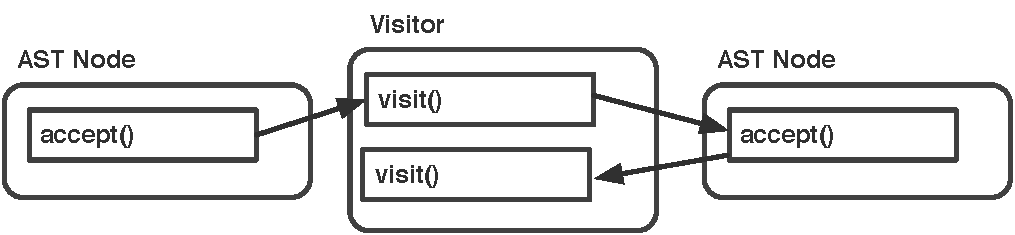
\includegraphics[scale=.60]{figures/flawed_visitor_organization.pdf}
\caption{A high level look at the organization of the flawed visitor.}
\label{fig:flawedvisitororganization}
\end{figure}

The reason for the appearance of this critical flaw is not certain to us who inherited this legacy code, but it seems likely to be related to having a singular visit method rather than pre and post visits. Having only one visit method per tree node restricts the traversal to only a pre-ordering or a post-ordering. \ref{fig:flawedvisitorexample} demonstrates a common scenario for AST traversal--the opening and closing of new scopes in the symbol table--which requires both orderings. The scope is opened as we traverse down the tree and closed as we traverse back up, but of course, this is not possible if we visit the node only once. The legacy code ``solves" this problem by placing the traversal logic inside the visitor methods and, in the process, defeats the very purpose of the visitor pattern. It is possible to reclaim a proper visitor pattern implementation by adding preorder and postorder visits. Consider the code with that minor change, shown in \ref{fig:fixedvisitorexample}

\begin{figure}[!htb]
\centering
\begin{minipage}{.45\textwidth}
\begin{lstlisting}[language=java]
public abstract
	class ResolveConceptualVisitor {
    preProcedureDecl(ProcedureDecl e) {}
    postProcedureDecl(ProcedureDecl e) {}
}

public abstract
	class ResolveConceptualElement {
    abstract void accept(
        ResolveConceptualVisitor e);
}

public class ProcedureDecl
	extends ResolveConceptualElement {	
    List<Stmt> myStatements;

    public void accept(
    	  ResolveConceptualVisitor e) {
        v.preProcedureDecl(this);
        for (Stmt s : e.getStatements()) {
            s.accept();
        }
        v.postProcedureDecl(this);
    }
}
\end{lstlisting}
\end{minipage}\quad
\begin{minipage}{.45\textwidth}
\begin{lstlisting}[language=java]
public abstract class Stmt
	extends ResolveConceptualVisitor {
    abstract void accept(
    	ResolveConceptualVisitor e) {}
}

public class Analyzer
	extends ResolveConceptualElement {
	
    public void preProcedureDecl(
  			ProcedureDecl e) {
        table.beginProcedureScope();
    }

    public void postProcedureDecl(
    			ProcedureDecl e) {
        table.endProcedureScope();
    }
}
\end{lstlisting}
\end{minipage}
\caption{A flawed implementation of the visitor pattern.}
\label{fig:fixedvisitorexample}
\end{figure}

\begin{figure}[!htb]
\centering
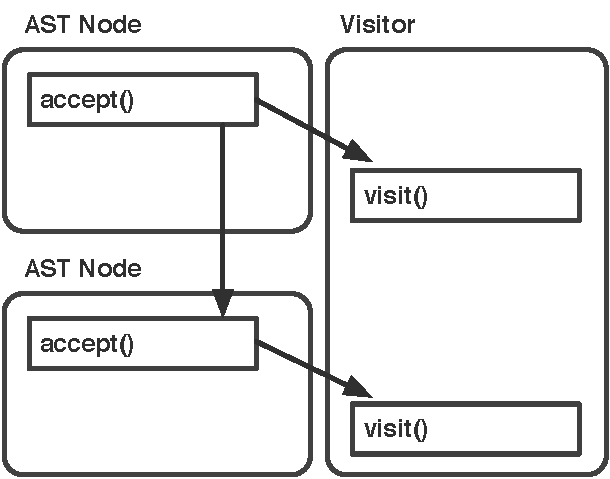
\includegraphics[scale=.60]{figures/fixed_visitor_organization.pdf}
\caption{A high level look at the organization of the fixed visitor.}
\label{fig:fixedvisitororganization}
\end{figure}

The \texttt{ResolveConceptualVisitor} now has fewer methods and the traversal logic is properly decoupled from the visitation logic.

% -----------------------------------------------------------------------------------------------
%	Contribution
% -----------------------------------------------------------------------------------------------

\section{A Dynamic Tree Walker}
While the corrections demonstrated in \ref{fig:fixedvisitororganization} could be made, we needed a solution that would not require refactoring of our legacy code. Our existing components needed to continue to work in their present form while we developed new versions of these components. Additionally we believed we could develop a solution that would consume much less time, both initially and in the long-term, than a significant refactoring would. Therefore we decided to pursue a third, even more robust implementation that would exist independently of--and work simultaneously with--legacy code.

The solution involves the creation of two new classes: \texttt{TreeWalker} and \texttt{TreeWalkerVisitor}. \texttt{TreeWalker} is the new traversal mechanism which is completely decoupled from both the tree structure and the visitation logic. It dynamically analyzes the tree composition at runtime using Java reflection. This \texttt{TreeWalkerVisitor} replaces the old \texttt{ResolveConceptualVisitor} class and provides a new abstract visitor class to implement visitor logic for the various components in the compiler. This design does not modify any existing code and still utilizes the \texttt{ResolveConceptualElement} AST classes. This allows the legacy code to continue to work alongside the new dynamic traversal component. In other words, old components can continue to work until new components are ready to be dropped in place.

With this new design, \texttt{TreeWalker} will dynamically analyze the structure of the tree at runtime and invoke the appropriate visitor methods as it traverses the tree. \ref{fig:newvisit} is a highly simplified version of the traversal algorithm code (see \ref{app:codelistings} for complete code).

\begin{figure}[!htb]
\centering
\begin{minipage}{.80\textwidth}
\begin{lstlisting}[language=java]
public void visit(ResolveConceptualElement e) {
    invokeVisitorMethods("pre", e);

    for (ResolveConceptualElement node : e.getChildren()) {
        visit(node);
    }
    invokeVisitorMethods("post", e);
}
\end{lstlisting}
\end{minipage}
\caption{A revised \texttt{visit} method.}
\label{fig:newvisit}
\end{figure}

The \texttt{visit} method is a simple recursive, depth-first traversal of the AST. At each level, the procedure will make ``pre" call before visiting children and a ``post" call after. These calls are made via \texttt{invokeVisitorMethods} -- a local method used to construct the appropriate visitor method name and dispatch the correct calls using reflection techniques (the details are not relevant to the overall design, but see \ref{app:codelistings} for this method's code). These calls include pre and post methods for each class (base and derived classes) represented by the AST node object.

\begin{figure}[!htb]
\centering
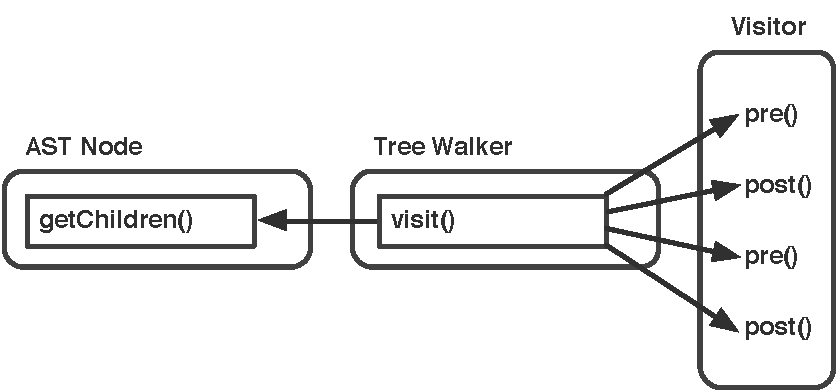
\includegraphics[scale=.60]{figures/prepostprepost.pdf}
\caption{A revised \texttt{visit} method.}
\end{figure}

The logic for retrieving a node's children is contained in the \texttt{getChildren} defined in the root AST class hierarchy, using the base \texttt{ResolveConceptualElement} class. This design choice allows for more control over the order of traversal. The default base method uses Java reflection to obtain a list of the children for a given node and returns the children in a list of unspecified order. Figure 4 shows a simplified version of this dynamic \texttt{getChildren} method (see \ref{app:codelistings} for complete code). If the order is important (or needs to be different from the default), then derived classes can override the method with static logic for returning the children.

\begin{figure}[!htb]
\centering
\begin{minipage}{.80\textwidth}
\begin{lstlisting}[language=java]
public List<ResolveConceptualElement> getChildren() {
    List<ResolveConceptualElement> children = new LinkedList<>();
    ArrayList<Field> fields = this.getDeclaredFields();
    
    for (Field field : fields) {
        if (ResolveConceptualElement.class.isAssignableFrom(field.getType())) {
            children.add(ResolveConceptualElement.class.cast(field.get(this)));
        }
    }
    
    return children;
}
\end{lstlisting}
\end{minipage}
\caption{An implementation of \texttt{getChildren}.}
\label{fig:getchildren}
\end{figure}


Use of the dynamic tree walker is simple and straightforward. To traverse an AST and apply appropriate visitation logic, first create an instance of the \texttt{TreeWalker} class, passing an instance of a \texttt{TreeWalkerVisitor} (such as the populator or code generator) as a parameter to the constructor. Then, simply call \texttt{visit} on the root of the abstract syntax tree.

% -----------------------------------------------------------------------------------------------
%	Results and Benefits
% -----------------------------------------------------------------------------------------------

% Blair: Read page 722 this link ("reflective visitor pattern") -- should be very helpful:
%http://onlinelibrary.wiley.com/store/10.1002/spe.2167/asset/spe2167.pdf?v=1&t=i0ofdec2&s=970e832ce7d5ec71bad48d4aca1eff81f2e26c8d
\section{Results and Benefits}

The dynamic tree walker is a unique and innovative reengineering approach that has yielded a number of benefits for our ongoing research project. The initial benefit was its rapid implementation. The original version of the dynamic tree walker, while admittedly less complex than the iteration seen in the appendix, was implemented by a single developer in the span of a few hours. This allowed us to begin work on new versions of our compiler components with very little delay and with no interruption to its existing operation. In fact, it allowed for simultaneous operation of both new and old components--each sharing the same AST class hierarchy but using their distinct tree traversal mechanisms.

Another major benefit of the dynamic tree walker is that it adds an entirely new layer of abstraction to the visitor pattern. The visitor pattern already mandates the decoupling of the traversal logic from the visitation logic, but our design also separates the traversal logic from the structure of the tree itself. Because the structure of the tree is extracted from the code dynamically at runtime, changes can be made to the AST classes and the tree walker will seamlessly adjust. The visitors, on the other hand, may need to be adjusted in cases where an existing part of the tree was renamed or removed--though perhaps not when adding to the tree. This is due to the fact that visitation logic is, by necessity, coupled with the tree structure.

In many compiler compilers, the relationship between the traversal algorithm and the tree structure is established in a pre-runtime code generation phase. This is usually accomplished by auto-generating AST classes with hard-coded traversal logic extracted from a grammar or other definition file. Our reengineering approach, however, does not require us to rewrite our legacy AST classes (or any part of them). Furthermore, it largely avoids the code generation step. It may be desirable to generate the abstract \texttt{TreeWalkerVisitor} class ahead of runtime to simplify the creation of new components by providing method declarations to override (indeed, we have opted for this approach). However, because methods are invoked using dynamically-constructed method names, this is not strictly necessary.

Finally, the dynamic tree walker is has reusable and maintainable. As has been clearly demonstrated, there is very little coupling in our design. This allows the tree walker to be effortlessly reused for any number of components in our compiler. The maintainability is also enhanced by the fact that the traversal logic is contained within a single class rather than distributed over the set of all AST classes. We have already leveraged this benefit by easily making additions and changes to the traversal such as inserting virtual nodes on-the-fly. Overall, the dynamic tree walker has saved a large amount of development time by eliminating the need to rewrite legacy code while also providing a rapidly implementable mechanism for continued iteration and evolution of the software.

% -----------------------------------------------------------------------------------------------
%	Application
% -----------------------------------------------------------------------------------------------

\section{Application Example: Code Generation}
\vspace{-2pt}

One important application of the walking mechanism described, concerns code generation. Since development began on the RESOLVE compiler, code generation -- like the many other phases of compilation -- was hindered not only by design of the initial AST visitor, but also by the (unusually) steep set of constraints we require in any prospective code generation system, including the following.

\begin{enumerate}
\item \textit{Correct by construction}: Provided with successfully verified RESOLVE source-code, it is the translator's responsibility to model, as faithfully as possible, each construct of the source language \textit{within} the target language. This modeling process -- performed to maintain the established correctness of the original source -- typically precludes the possibility of any sort of syntax-directed translation, as any code generated fitting such a model inevitably ends up looking wildly different from the original source.
\item \textit{Extensibility}: The design of the translator must allow users to relatively easily tweak the output of a given construct, add support for altogether new constructs (accounting for the rapidly developing nature of the source language), and not preclude the addition of any future target languages. This is ultimately one of the reasons we choose to perform source-to-source translation, as opposed generating byte code such as JVM or LLVM single static assignment form directly: It allows a certain level of flexibility -- leaving us free to temporarily sidestep the non-trivial problem of developing (and maintaing) a fully blown byte level interpretation of every construct, in favor of more fruitful, verification related avenues of research.
\item \textit{Reusability}: If two or more supported target languages share similar constructs, the (separate) modules responsible for generating code for each should not duplicate code. Rather, they would ideally be designed to share as much common translation logic as possible, typically via an abstract class or some other means. However, if this is to occur, the translator in question must be designed in such a way that it enforces a strict separation between the logic governing the collection of translation related information, and the actual formatted output of this information.
\end{enumerate}

In this section we detail -- by way of a small example -- our approach that combines the pre-post visit methods of the tree walker, with the Antlr-authored templating tool, \textit{Stringtemplate}\footnote[3]{\texttt{www.theantlrguy.atlassian.net/wiki/display/ST4/StringTemplate+4+Documentation}} \cite{parr:2006}.

\subsection{Stringtemplate Overview}
In order to better understand the example that follows, we provide a brief overview of the Stringtemplate language, emphasizing its notation, and usage. A popular `definition' of a template describes it simply as a ``document with holes" that users can choose to fill with \textit{attributes}. For instance, the following is a template describing a RESOLVE variable declaration.
\begin{lstlisting}
VarDecl(name, type) ::= "Var <name> : <type>;"
\end{lstlisting}

In this case, \texttt{name} and \texttt{type} serve as attributes to this template, and are to be substituted where they appear within the angled braces (\texttt{<..>}) in the text. In order to interact with this template, users can obtain a reference to it, assign its attributes, and print it out -- demonstrated in Listing \ref{listing:stringtemplate_fill}.

\begin{lstlisting}[caption={Basic template manipulation.},label={listing:stringtemplate_fill}]
//A 'group' is collection of templates defined in an external file
ST variableDecl = myGroup.getInstanceOf("VarDecl"); 

//We fill in the attributes for 'name' and 'type'
variableDecl.add("name", "X");
variableDecl.add("type", "Integer");		     

//Then render the overall template (ST) and print the resulting string
System.out.println(variableDecl.render());

//Result:
>$ Var X : Integer;
\end{lstlisting}

If however we wanted to modify our template to correctly account for declarations involving two or more variables of the same type, we could simply tweak the template's definition to read as follows.

\begin{lstlisting}
VarDecl(name, type) ::= "Var <name; separator = ', '> : <type>;"
\end{lstlisting}

This small change instructs Stringtemplate to interpret any \textit{multi-valued} attribute passed as a comma delimited list. For instance, if the addition of \texttt{name} in the previous example was replaced with,

\begin{lstlisting}[language=java]
variableDecl.add("name", "X").add("name", "Y");
\end{lstlisting}	

Stringtemplate would yield the following output.
\begin{lstlisting}[language=java]
>$ Var X, Y : Integer;
\end{lstlisting}

This section only provides readers with the bare minimum knowledge required to understand the discussion of translation that follows. Readers interested in learning more about this tool are encouraged to refer to \cite{parr:2006} or \cite{parr:2004}.

\subsection{RESOLVE Module Translation}

To better understand the tree walker's key role in RESOLVE's code generation, we consider the trivial operation in Listing \ref{listing:example_operation}.

\begin{lstlisting}[caption={A RESOLVE example operation.},label={listing:example_operation}]
Operation Foo(evaluates J: Integer);
Procedure
	Bar(J);
end Foo;
\end{lstlisting}

There is little needed to translate \texttt{Foo} into Java (or C) for execution. In fact, the translator class hierarchy (depicted in Figure \ref{fig:translation_uml}) only needs to maintain global reference to a stack of partially filled in, intermediate templates representing various levels traversed of the AST, and the file from which to obtain new, target-language specific templates.

\begin{figure}[!htb]
\centering
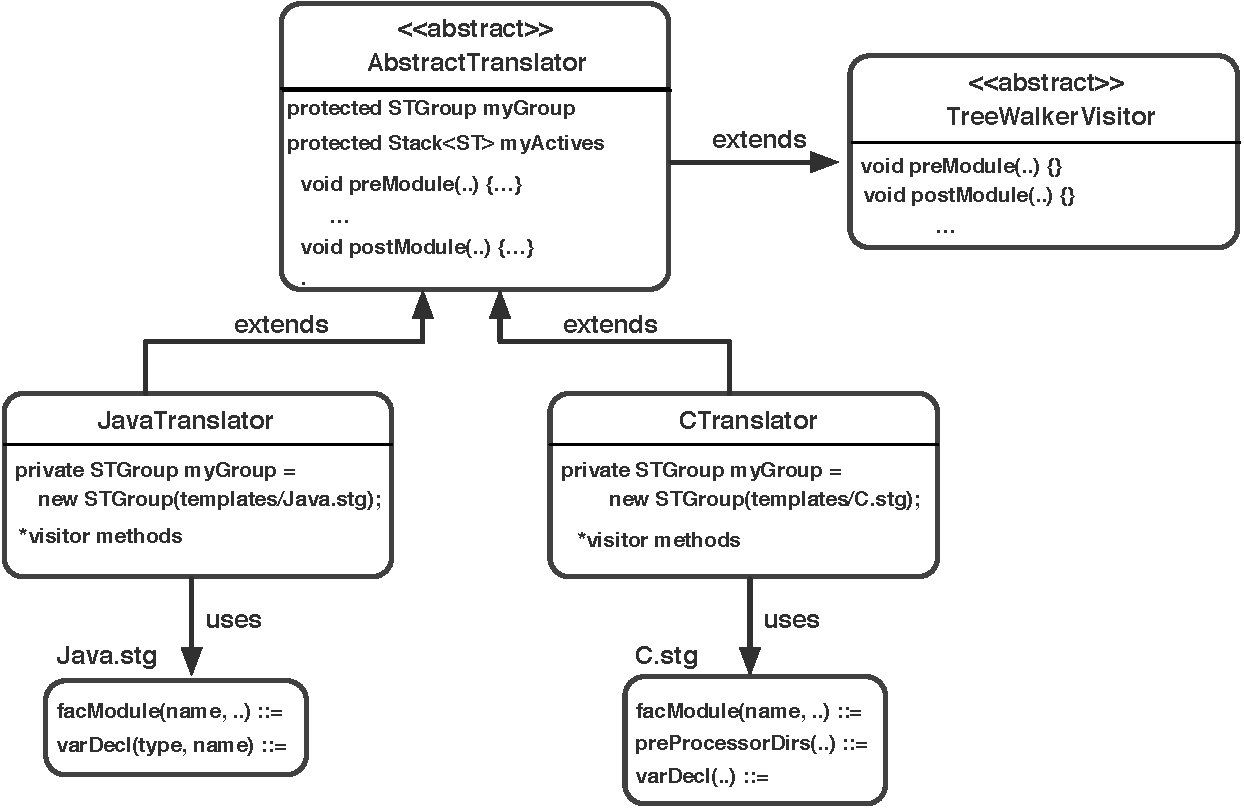
\includegraphics[scale=.40]{figures/translation_uml.pdf}
\caption{RESOLVE's translation hierarchy. Each concrete subclass of the abstract translator has an accompanying, dedicated Stringtemplate group file containing all templates tailored to the target language of the class.}
\label{fig:translation_uml}
\end{figure}

The first step we take in this process is to define a set of templates which -- when rendered -- output a Java representation of the original RESOLVE code. Listing \ref{listing:required_templates} summarizes all the templates we require, including those for functions, parameters, calls, variable arguments, and, at the most granular: (potentially) qualified types.\footnote{It turns out that many templates as they appear in Listing \ref{listing:required_templates} (such as\texttt{FunctionDefinition}), are suitable for both Java and C output. Thus, to avoid duplication at the template-level, we actually declare templates such as these in a separate template group file that plays the role of an `abstract-template-group,' from which our dedicated C and Java groups inherit.}.

\begin{lstlisting}[caption={Templates required for translation of our example. Note: Templates wrapped by ``\texttt{<<..>>}" indicate that whitespace, newlines, and tabs are to be preserved.},label={listing:required_templates}]
//functions
FunctionDefinition(name, type, parameters, vars, statements) ::= <<			
public <type> <name> (<parameters; sep=', '>) {
	<statements; separator='\n'>
}>>

//parameter declarations
ParameterDecl(type, name) ::= "<type> <name>"

//call statements
CallStmt(qualifier, name, args) ::= "<if(qualifier)>.<endif><name>(<args; sep=', '>);"

//variable expressions
VarExp(qualifier, name) ::= "<name>"

//type
type(qualifier, name) ::= "<if(qualifier)>.<endif><name>"
\end{lstlisting}

It's now up to the Java Translator to completely ``fill" the \texttt{name}, return \texttt{type}, \texttt{parameters}, and \texttt{statements} attributes of the \texttt{FunctionDefinition} template -- either using strings, or other filled-in, templates. One effective way to do so -- that we now demonstrate -- involves simply using a stack, and the tree walker's pre-post traversal. 

\begin{figure}
\centering
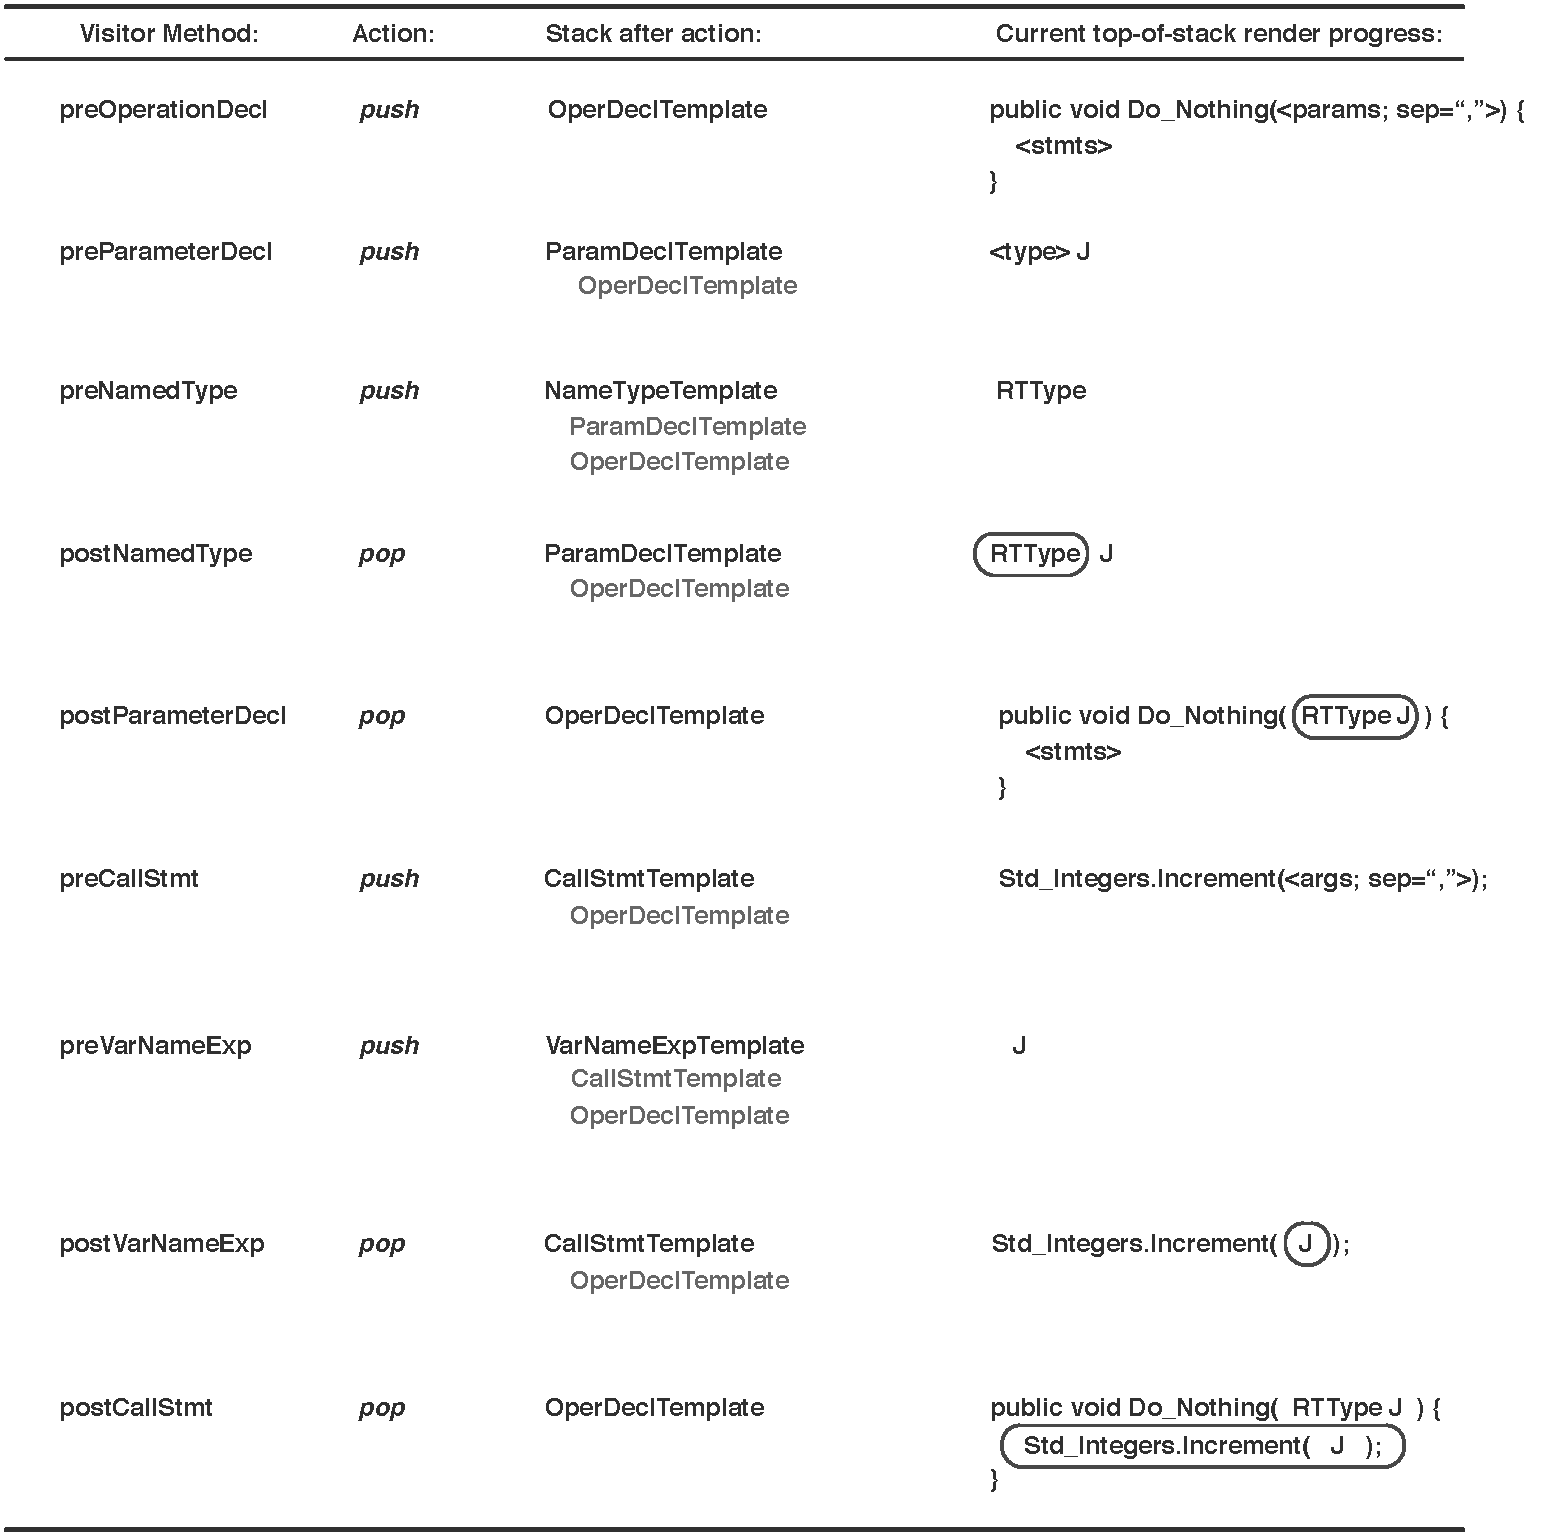
\includegraphics[scale=.50]{figures/translation_table.pdf}
\caption{A table illustrating the translation of operation \texttt{Foo}. MORE}
\label{fig:translation_flow}
\end{figure}

The table depicted in Figure \ref{fig:translation_flow} illustrates both the order and state of the translation template stack over the course of the AST's traversal. At every stage of translation, the top of this stack maintains a reference to the template actively being built, or added to, while the bottom always refers to the result (or, the outermost enclosing template that is to be rendered upon completion). 

Thus, translation of any given for any given target language is performed as follows:
\begin{enumerate}
\item In the context of a pre$C$ visitor method (where $C$ corresponds to some RESOLVE construct), we first retrieve $C$'s corresponding template, $T$, from the current translation subclass's template group file. We then pass any easily obtainable information from $C$'s AST node into $T$ as attributes. Finally, we push $T$ onto the global template stack.

\item Over course of traversing $C$'s children, we modify the top of this stack arbitrarily -- filling in any additional attributes. However, in the event that a child, $C'$, is as complicated as $C$, we perform the same steps as in (1), pushing a new template $T'$ representing $C'$ onto the stack, and walking its respective children.

\item In post visitor methods (post$C$), we simply pop the completed entry off the stack, and either print it out (if we're done) or add it as an appropriate attribute to the new/current top of the stack.
\end{enumerate}

We have found the tree walker to be an invaluable asset to this process, as not only does the pre and post for each construct allow us to produce arbitrarily complicated, nested block of structured output, but also provides a valuable context that allows us to keep translation forwarding logic separate from the nitty, gritty details of output. 

In summary, the only actual work being performed within the translator is forwarding information collected from individual \texttt{ResolveConceptualElement}s, to a series of externally defined templates. This allows us to exploit (in design pattern parlance) a strict model view controller (MVC) separation in the translator's codebase between the mechanism that does the AST visiting (controller), the individual \texttt{ResolveConceptualElement}s from which we're forwarding information to templates (model), and the external file containing all available C or Java language templates which shape our output (view) \cite{parr:2004,krasner:1988}.

%Translation itself is performed over the course of a walk of the AST that represents the code in \ref{fig:int_do_nothing}. Ideally, according to our constraints above, we would like a means of maximizing the amount of code shared between our two currently supported target languages (Java and C). 

%This module 
%Shown in \ref{fig:translationflow} is a high level depiction of the steps taken in translating this operation to C. The first box depicts the AST of operation \texttt{Int\_Do\_Nothing}, where nodes are represented as boxes labeled by the constructs they contain. Throughout the walk of the tree, useful information such as the operation's name ``Int\_Do\_Nothing" are extracted from the nodes, and added as parameters to user defined templates, in this case: \texttt{c\_function\_def}.

%\begin{figure}
%\centering
%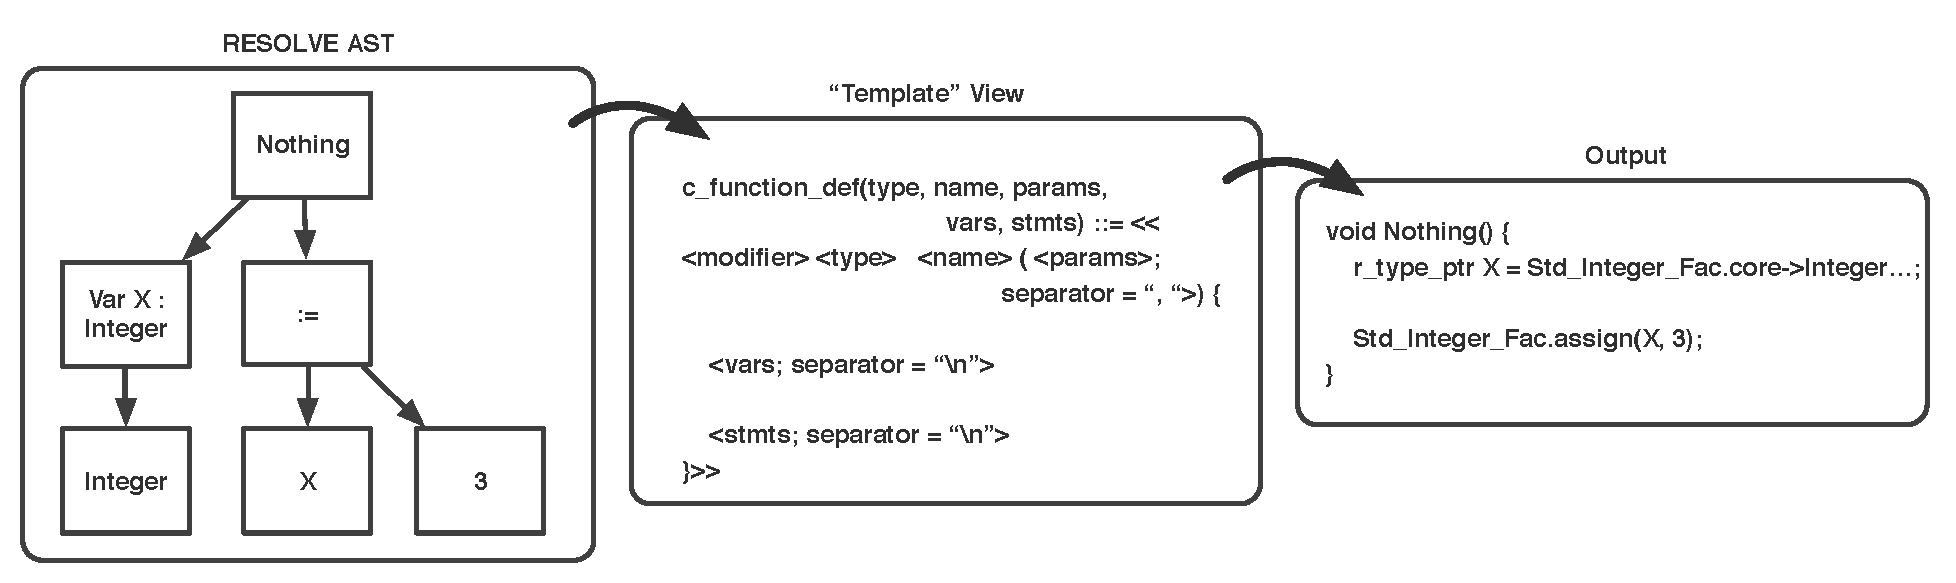
\includegraphics[scale=.40]{figures/ast_traversal2.pdf}
%\caption{The general flow of information from the AST (first), to user defined templates (middle), ending with formed output (last).}
%\label{fig:translationflow}
%\end{figure}

%In the context of RESOLVE to C translation, these templates, when filled during the aforementioned pre-post visitor traversal of RESOLVE's AST, help simplify the task of producing arbitrarily complicated, nested blocks of structured C output by keeping translation logic strictly with the C translator, and output logic strictly within the templates.

%

%We feel the approach to tree walking in the paper lends itself well to this strategy of translation, as this separation allows us to easily iterate changes to our generated C (or Java!) code without needing to concern ourselves with the compiler or translator itself.

% -----------------------------------------------------------------------------------------------
%	Conclusion
% -----------------------------------------------------------------------------------------------

\section{Conclusion}

% -----------------------------------------------------------------------------------------------
%	Acknowledgments
% -----------------------------------------------------------------------------------------------

\section{Acknowledgements}

\bibliography{treewalkreferences}

% -----------------------------------------------------------------------------------------------
%	Appendices
% -----------------------------------------------------------------------------------------------

\newpage
\section{Appendix} \label{app:codelistings}
\begin{lstlisting}[language=java,caption={TreeWalker.java}]
public class TreeWalker {

    private TreeWalkerVisitor myVisitor;

    /**
     * Constructs a new <code>TreeWalker</code> that applies the logic of
     * <code>TreeWalkerVisitor</code> to a RESOLVE abstract syntax tree.
     * @param twv	An instance of TreeWalkerVisitor which implements
     * 				visitor methods to be applied to nodes of the AST.
     */
    public TreeWalker(TreeWalkerVisitor visitor) {
        this.myVisitor = visitor;
    }

    /**
     * Visits the node <code>e</code> by calling pre- visitor methods, recursively
     * visiting child nodes, and calling post- visitor methods.
     * If the <code>TreeWalkerVisitor</code> contains a method named
     * <code>walk[className]</code>, that method is called instead of visiting the children.
     * @param e	The RESOLVE abstract syntax tree node to visit/walk
     */
    public void visit(ResolveConceptualElement e) {
        if (e != null) {
            // are we overriding the walking for this element?
            if (!walkOverride(e)) {
                // invoke the "pre" visitor method(s)
                invokeVisitorMethods("pre", e);

                java.util.List<ResolveConceptualElement> children =
                        e.getChildren();

                if (children.size() > 0) {
                    Iterator<ResolveConceptualElement> iter =
                            children.iterator();

                    ResolveConceptualElement prevChild = null, nextChild = null;
                    while (iter.hasNext()) {
                        prevChild = nextChild;
                        nextChild = iter.next();
                        invokeVisitorMethods("mid", e, prevChild, nextChild);
                        visit(nextChild);
                    }
                    invokeVisitorMethods("mid", e, nextChild, null);
                }
                // invoke the "post" visitor method(s)
                invokeVisitorMethods("post", e);
            }
        }
    }

    private void invokeVisitorMethods(String prefix,
            ResolveConceptualElement... e) {
        boolean pre = prefix.equals("pre"), post = prefix.equals("post"), mid =
                prefix.equals("mid"), list = (e[0] instanceof VirtualListNode);

        // Invoke generic visitor methods (preAny, postAny)
        if (pre) {
            myVisitor.preAny(e[0]);
        }

        // Get the heirarchy of classes from which this node inherits
        // e.g., [ConceptModuleDec, ModuleDec, Dec, ResolveConceptualElement]
        Class<?> elementClass = e[0].getClass();
        ArrayList<Class<?>> classHierarchy = new ArrayList<Class<?>>();

        if (list) {
            classHierarchy.add(((VirtualListNode) e[0]).getParent().getClass());
        }
        else if (pre || post) {
            while (elementClass != ResolveConceptualElement.class) {
                if (post) {
                    classHierarchy.add(elementClass);
                }
                else {
                    classHierarchy.add(0, elementClass);
                }
                elementClass = elementClass.getSuperclass();
            }
        }
        else {
            classHierarchy.add(elementClass);
        }

        // Iterate over the class hierarchy
        Iterator<Class<?>> iter = classHierarchy.iterator();
        while (iter.hasNext()) {
            Class<?> currentClass = iter.next();

            // Construct name of method
            String className, methodName;
            if (!list) {
                className = currentClass.getSimpleName();
            }
            else {
                className = ((VirtualListNode) e[0]).getNodeName();
            }
            methodName = prefix + className;

            ResolveConceptualElement[] parent = Arrays.copyOf(e, e.length);
            // Get parent and child types if this is a list node
            Class<?> paramType = ResolveConceptualElement.class;
            if (list) {
                paramType = ((VirtualListNode) e[0]).getListType();
                parent[0] = ((VirtualListNode) e[0]).getParent();
            }

            // Now try to obtain the proper visitor method
            try {
                Method visitorMethod;
                if (pre || post) { // pre and post methods
                    visitorMethod =
                            this.myVisitor.getClass().getMethod(methodName,
                                    currentClass);
                }
                else { // mid methods
                    visitorMethod =
                            this.myVisitor.getClass().getMethod(methodName,
                                    currentClass, paramType, paramType);
                }

                // Invoking the visitor method now!
                visitorMethod.invoke(this.myVisitor, (Object[]) parent);
            }
            catch (NoSuchMethodException nsme) {
                //This is fine if we're dealing with a virtual node,
                //otherwise it shouldn't be possible
                if (!list) {
                    throw new RuntimeException(nsme);
                }
            }
            catch (IllegalAccessException iae) {
                throw new RuntimeException(iae);
            }
            catch (InvocationTargetException ite) {
                Throwable iteCause = ite.getCause();

                if (iteCause instanceof RuntimeException) {
                    throw (RuntimeException) iteCause;
                }

                throw new RuntimeException(iteCause);
            }
        }

        if (post) {
            myVisitor.postAny(e[0]);
        }
    }

    private boolean walkOverride(ResolveConceptualElement e) {
        Class<?> elementClass = e.getClass();
        ArrayList<Class<?>> classHierarchy = new ArrayList<Class<?>>();
        while (elementClass != ResolveConceptualElement.class) {
            classHierarchy.add(0, elementClass);
            elementClass = elementClass.getSuperclass();
        }

        boolean foundOverride = false;
        Iterator<Class<?>> iter = classHierarchy.iterator();
        while (iter.hasNext() && !foundOverride) {
            Class<?> c = iter.next();

            if (!c.equals(VirtualListNode.class)) {
                String walkMethodName = "walk" + c.getSimpleName();
                try {
                    Method walkMethod =
                            this.myVisitor.getClass().getMethod(walkMethodName,
                                    c);
                    foundOverride =
                            ((Boolean) walkMethod.invoke(this.myVisitor, e));
                }
                catch (NoSuchMethodException nsme) {
                    //Shouldn't be possible
                    throw new RuntimeException(nsme);
                }
                catch (IllegalAccessException iae) {
                    //Shouldn't be possible
                    throw new RuntimeException(iae);
                }
                catch (InvocationTargetException ite) {
                    //An exception was thrown inside the corresponding walk method
                    Throwable iteCause = ite.getCause();

                    if (iteCause instanceof RuntimeException) {
                        throw (RuntimeException) iteCause;
                    }

                    throw new RuntimeException(iteCause);
                }
            }
        }
        return foundOverride;
    }
}
\end{lstlisting}

\begin{lstlisting}[language=java,caption={TreeWalkerVisitor.java}]
public abstract class TreeWalkerVisitor {
    // AbstractFunctionExp
    public boolean walkAbstractFunctionExp(AbstractFunctionExp data) {
        return false;
    }

    public void preAbstractFunctionExp(AbstractFunctionExp data) {}

    public void midAbstractFunctionExp(AbstractFunctionExp node,
            ResolveConceptualElement previous, ResolveConceptualElement next) {}

    public void postAbstractFunctionExp(AbstractFunctionExp data) {}
    
    // Continue for all types of AST nodes... 
}

\end{lstlisting}

\begin{lstlisting}[language=java,caption={ResolveConceptualElement.java}]

public abstract class ResolveConceptualElement {
    public List<ResolveConceptualElement> getChildren() {

        //We'd like to hit the fields in the order they appear in the class,
        //starting with the most general class and getting more specific.  So,
        //we build a stack of the class hierarchy of this instance
        
        Deque<Class<?>> hierarchy = new LinkedList<Class<?>>();
        Class<?> curClass = this.getClass();
        do {
            hierarchy.push(curClass);
            curClass = curClass.getSuperclass();
        } while (curClass != ResolveConceptualElement.class);

        List<ResolveConceptualElement> children = new List<ResolveConceptualElement>();
        ArrayList<Field> fields = new ArrayList<Field>();
        while (!hierarchy.isEmpty()) {

            curClass = hierarchy.pop();

            Field[] curFields = curClass.getDeclaredFields();
            for (int i = 0; i < curFields.length; ++i) {
                fields.add(curFields[i]);
            }
            curClass = curClass.getSuperclass();
        }

        // loop through all the class members
        Iterator<Field> iterFields = fields.iterator();
        while (iterFields.hasNext()) {
            Field curField = iterFields.next();
            if (!Modifier.isStatic(curField.getModifiers())) {
                curField.setAccessible(true);
                Class<?> fieldType = curField.getType();

                try {
                    // is this member a ResolveConceptualElement?
                    // if so, add it as a child
                    if (ResolveConceptualElement.class
                            .isAssignableFrom(fieldType)) {
                        //System.out.println("Walking: " + curField.getName());
                        children.add(ResolveConceptualElement.class
                                .cast(curField.get(this)));
                    }
                    // is this member a list of ResolveConceptualElements?
                    // if so, add the elements to the list of children
                    else if (java.util.List.class.isAssignableFrom(fieldType)) {
                        Class<?> listOf =
                                (Class<?>) ((ParameterizedType) curField
                                        .getGenericType())
                                        .getActualTypeArguments()[0];
                        java.util.List<?> fieldList =
                                java.util.List.class.cast(curField.get(this));
                        if (fieldList != null
                                && fieldList.size() > 0
                                && ResolveConceptualElement.class
                                        .isAssignableFrom(listOf)) {
                            children
                                    .add(new VirtualListNode(
                                            this,
                                            curField.getName(),
                                            (java.util.List<ResolveConceptualElement>) fieldList,
                                            (Class<?>) ((ParameterizedType) curField
                                                    .getGenericType())
                                                    .getActualTypeArguments()[0]));
                        }
                    }
                }
                catch (Exception ex) {
                    if (ex instanceof RuntimeException) {
                        throw (RuntimeException) ex;
                    }
                    else {
                        throw new RuntimeException(ex);
                    }
                }
            }
        }

        return children;
    }
}
\end{lstlisting}

\end{document}
